\documentclass[hyperref={pdfpagelabels=false}]{beamer}
\usepackage{lmodern}
\usepackage{graphicx}
\usepackage{url}
\usetheme{PaloAlto}
\title{Graphical User Interface for Floor Plan Visualization at Allegheny College}  
\author{CeCe Col\'{o}n}
\date{November 20, 2017} 
\begin{document}
\logo{\includegraphics[scale=0.15]{ghenyLogo}}
\begin{frame}
\titlepage
\end{frame} 


\section{Motivation}
\hypertarget{Motivation}{{}}
%\subsection{Motivation}
\begin{frame}
\frametitle{Motivation}

\begin{columns}
	 \begin{column}{.45\textwidth}
\begin{itemize}[<+->]
\item Current Availability 
\item Data and information Visualization
\item Branding
\begin{itemize}
	\item New Applications
	\item Retention
\end{itemize} 
\item Rooming Information
\end{itemize} 
	\end{column}
 \begin{column}{.6\textwidth}
 	 \centering
             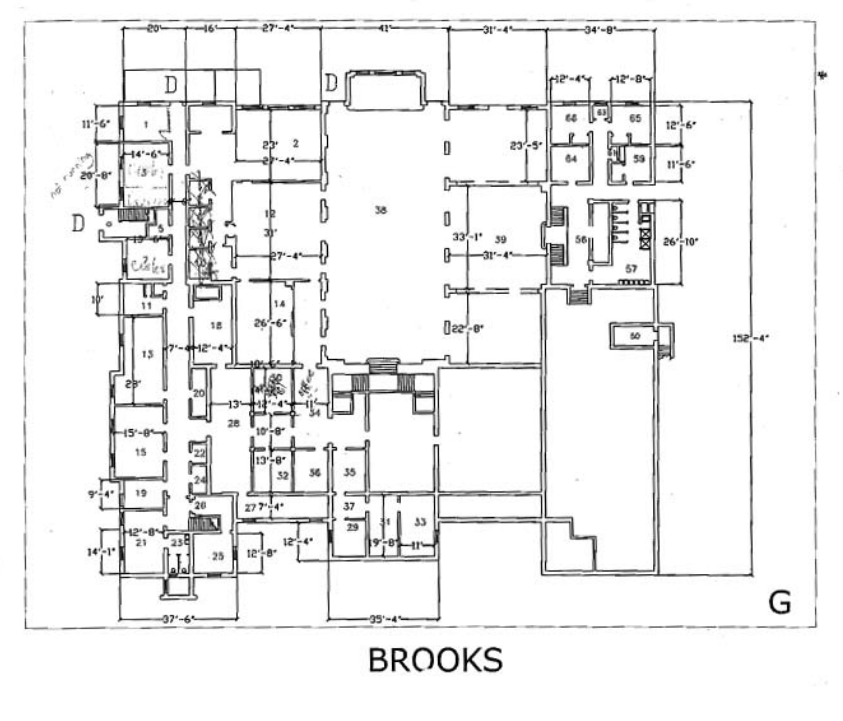
\includegraphics[height=5cm, width=5.5cm]{brooksG.png} 
 \end{column}

\end{columns}
\end{frame}
%%%%%%%%%%%%%%%%%%%%%%%%%%%%%%%%
\section{Solution} 
\hypertarget{Solution}{{}}
\begin{frame}
\frametitle{Solution}
\begin{itemize}[<+->]
	\item Graphical User Interface
	\item Interactivity
	\item SVG 2D floor plans 
	\item {\Large Goals}
	\begin{itemize}
		\item CLARITY and VISIBILITY
		\item Display relevant information
		\item Useful to different offices 
	\end{itemize}
\end{itemize}
\end{frame}
%%%%%%%%%%%%%%%%%%%%%%%%%%%%%%%%
\section{Related Work}
\hypertarget{Related Work}{{}}
\begin{frame}
\frametitle{Related Work}

\begin{columns}
	 \begin{column}{.5\textwidth}
\begin{itemize}[<+->]
	\item Paid Programs
	\begin{itemize}
		\item Campus Bird \url{http://map.allegheny.edu/}
		\item nuCloud
	\end{itemize}
	\item SVG country maps
	\item University Created Floor Plans
	\begin{itemize}
		\item \textbf{Case Western} 
		\item Rochester Institute of Technology
	\end{itemize}
\end{itemize}	 
\end{column}
	
 \begin{column}{.6\textwidth}
 	\centering
    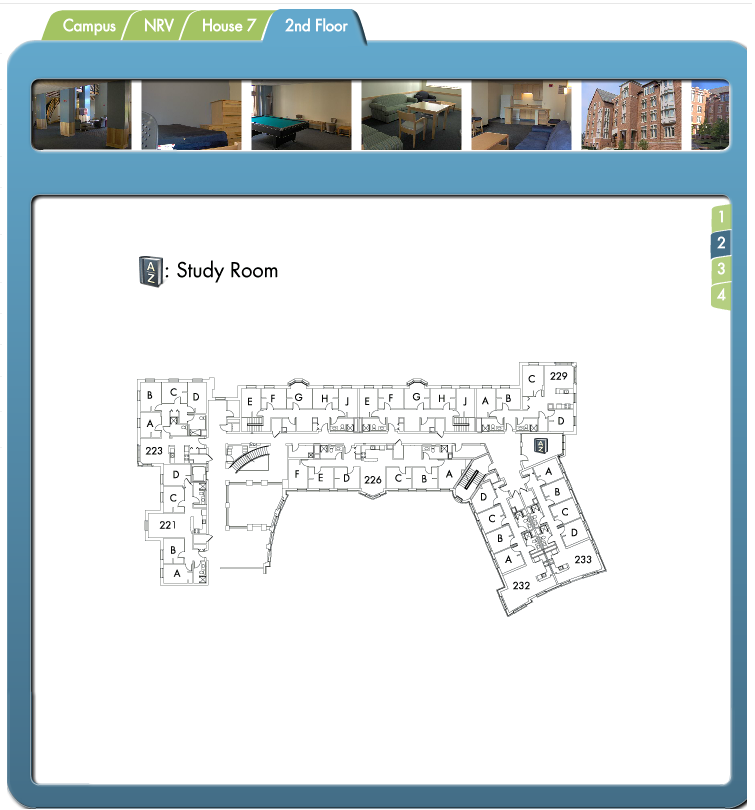
\includegraphics[height=5cm, width=5.5cm]{CWRUFacilitiesTourFloorPlan.png} 
 
 \end{column}

\end{columns}
\end{frame}
%%%%%%%%%%%%%%%%%%%%%%%%%%%%%%%%
\section{Approach} 
\hypertarget{Approach}{{}}
\begin{frame}
\frametitle{Approach}
\begin{itemize}[<+->]
	\item Convert current Floorplans to SVG graphics
	\begin{itemize}
		\item Adobe Illustrator
		\item InkScape
	\end{itemize}
		\item SVG code editing
		\item Adding Interactivity
	\begin{itemize}
		\item JavaScript
		\item HTML
	\end{itemize}
	\item Displaying all information in a fluid way
\end{itemize}
\end{frame}
%%%%%%%%%%%%%%%%%%%%%%%%%%%%%%%
\section{Why SVG?}
\hypertarget{Why SVG?}{{}}
%\subsection{Motivation}
\begin{frame}
\frametitle{SVG vs Everything Else}

\begin{columns}
	\begin{column}{.6\textwidth}
	\centering	
	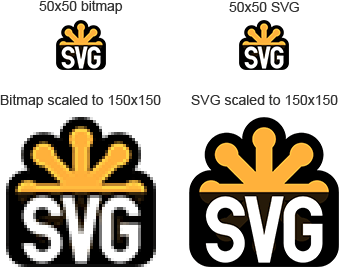
\includegraphics[height=4cm,width=5cm]{svgInfo.png} 
	\end{column}
 \begin{column}{.45\textwidth}
 	 \begin{itemize}[<+->]
 	 	\item XML-based vector graphic
 	 	\begin{itemize}
 	 			\item Compatible with HTML, JavaScript (JQuery), and CSS 
 	 		\end{itemize}
 	 		\item Scripting interactivity
 	 		\item D3.js, Snap.js, Raphael.js
 	 		\item No resolution limits
 	 		\item Faster load times
 	 \end{itemize}
 \end{column}
\end{columns}
\end{frame}
%%%%%%%%%%%%%%%%%%%%%%%%%%%%%%%%
\section{Evaluation Strategy} 
\hypertarget{Evaluation Strategy}{{}}
\begin{frame}
\frametitle{Evaluation Strategy}
\begin{itemize}[<+->]
	\item Manual Testing
	\item System Usability Scale (SUS)
		\begin{itemize}
			\item Standardized method of evaluation
		\end{itemize}
	\item Self Created Questionnaire
	\begin{itemize}
		\item Specific feedback in context for Allegheny
	\end{itemize}
\end{itemize}
\end{frame}
%%%%%%%%%%%%%%%%%%%%%%%%%%%%%%%%%
\section{Other} 
\hypertarget{Other}{{}}
\begin{frame}
\frametitle{Other Considerations}
\begin{itemize}
	\item Institutional Review Board Form
	\begin{itemize}
		\item Focus Group and Surveys to determine included information
		\item Survey for post floor plan evaluations
	\end{itemize}
\end{itemize}

\begin{table}[htbp]
  \centering
  \begin{tabular}{|c||c|c|}
    \hline
    \bf Task     & \bf Begin Date & \bf End Date \\ \hline\hline    
    Chapter 1 and 2 final draft & 20 Nov        & 12 Dec     \\ \hline
    Collecting original floor plans & 12 Dec   & 20 Dec      \\ \hline
    Creating SVG images	     & 20 Dec        & 15 Jan       \\ \hline
    Interactivity for SVG      & 15 Jan         & 15 Feb        \\ \hline
    Building Program Framework & 15 Feb 		 & 15 March		\\ \hline
    Evaluation/Debugging		& 15 March		 & 5 April		\\ \hline
    Final draft for edits	     & 1 April        & 20 April     \\ \hline
    Edits 			             & 20 April       & 27 April     \\ \hline
	Final, bound copy submitted & 27 April       & 1 May         \\ \hline
  \end{tabular}
  %\caption{Beakdown of Proposed Work Schedule}~\label{intro-tab1}
\end{table} 
\end{frame}
%%%%%%%%%%%%%%%%%%%%%%%%%%%%%
\section{Future Work} 
\hypertarget{Future Work}{{}}
\begin{frame}
\frametitle{Future Work - Extended Applications}
\begin{itemize}[<+->]
	\item Pelletier Library
	\begin{itemize}
		\item Stacks layout
		\item Study Rooms
		\item Public Computer Locations
	\end{itemize}
	\item Campus Programming Spaces
	\begin{itemize}
		\item Campus Center
		\item Shultz
		\item Tippie
	\end{itemize}
\end{itemize}
\end{frame}

\end{document}

